\documentclass[12pt]{article}
\usepackage[pdftex]{graphicx}
%\usepackage[body={190mm,277mm},top=10mm,left=10mm,nohead]{geometry}

%\documentclass[12pt]{article}
%\usepackage[utf8]{inputenc} % nastavuje pou�it� k�dov�n�, u�ivatel� Windows zam�n� latin2 za cp1250
%\usepackage[T1]{fontenc}
\usepackage{a4wide} % nastavuje standardn� evropsk� form�t str�nek A4
%%\usepackage{index} % nutno pou��t v p��pad� tvorby rejst��ku bal��kem makeindex
%%\usepackage{fancybox} % umo��uje pokro�il� r�me�kov�n� :-)
%\usepackage[pdftex]{graphicx} % nezbytn� pro standardn� vkl�d�n� obr�zk� do dokumentu
%\usepackage{enumerate}
%\usepackage{listings}
%\usepackage[dvips]{color}
\usepackage{subfigure}
%\usepackage{amssymb,amsmath

\setlength{\parindent}{0pt} 
\setlength{\parskip}{2ex}

\title{Solution for assignment \#1}
\date{October 27, 2012}
\author{Vojtech Kopal}

\newcommand{\mytilde}{\raise.17ex\hbox{$\scriptstyle\mathtt{\sim}$} }

\begin{document}

\maketitle

\clearpage

\section{Economic part}

\subsection*{a) Economic growth and convergence - descriptive statistics:}

\begin{figure}[h!]
  \centering           
  \subfigure{                         
  	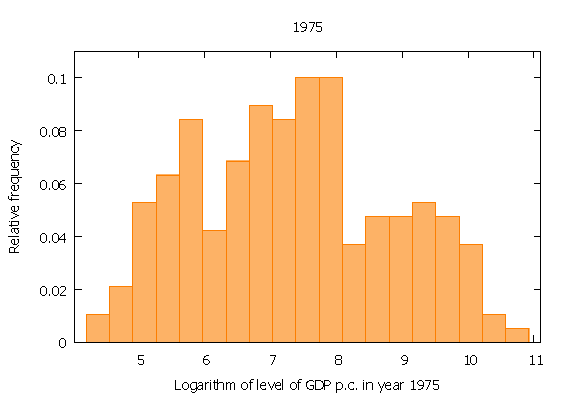
\includegraphics[scale=0.7]{parts/1a_1}
  	\label{1a:gpd1975}
  }                   
  \subfigure{                         
  	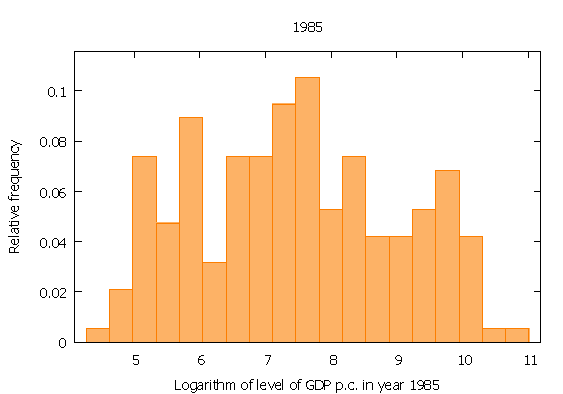
\includegraphics[scale=0.7]{parts/1a_2}
  	\label{1a:gpd1985}
  }                 
  \subfigure{                         
  	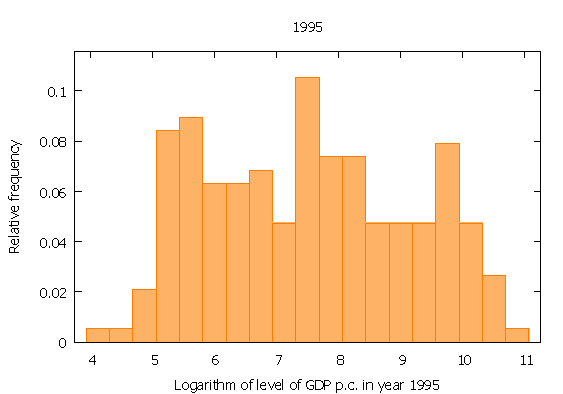
\includegraphics[scale=0.7]{parts/1a_3}
  	\label{1a:gpd1995}
  }                 
  \subfigure{                         
  	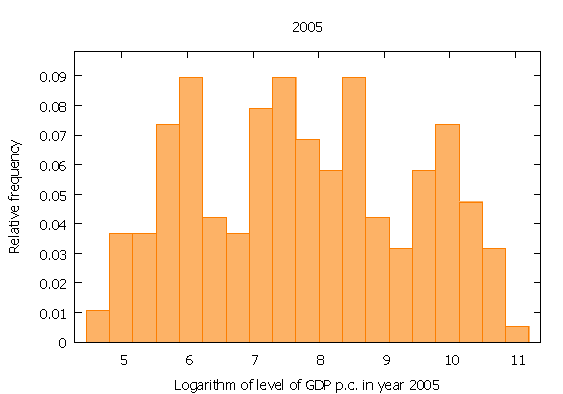
\includegraphics[scale=0.7]{parts/1a_4}
  	\label{1a:gpd2005}
  }                         
  \caption{The changes in distribution of GDP p.c. among 190 countries in years 1975, 1985, 1995 and 2005.}
\end{figure}

Omitting Djibouti.

Commenting on changes.

\clearpage

Median income in 1975 is 1487.6

Rich countries

\begin{figure}[h!]
  \centering           
  \subfigure{                         
  	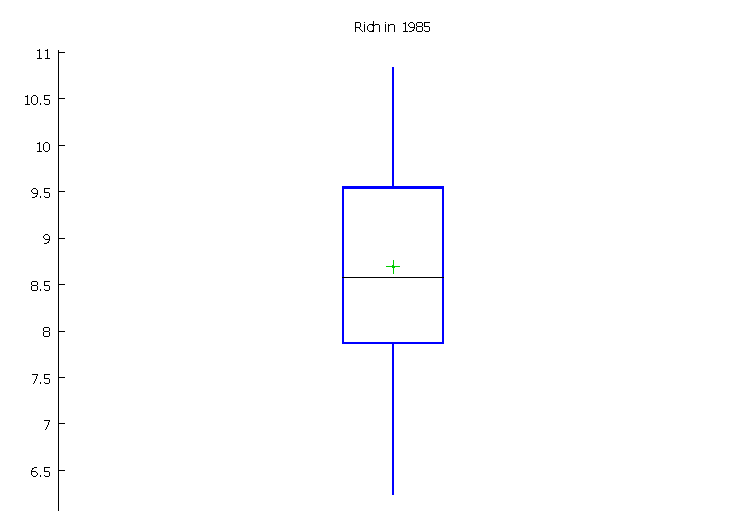
\includegraphics[scale=0.3]{parts/1a_5}
  	\label{1a:rich1985}
  }                   
  \subfigure{                         
  	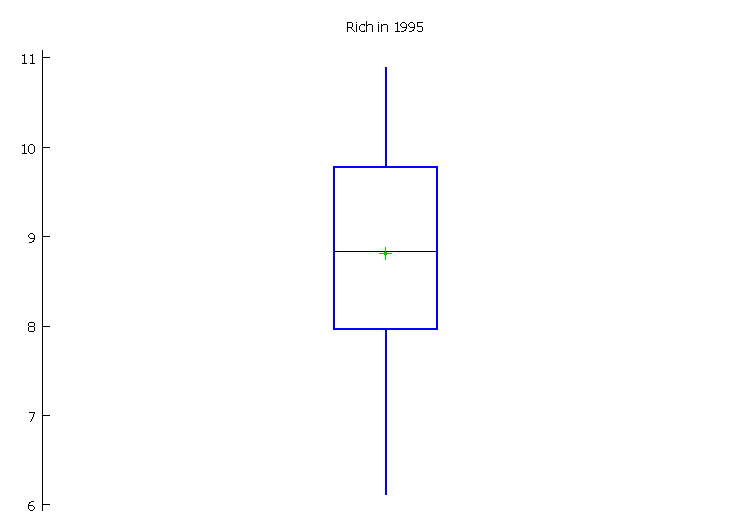
\includegraphics[scale=0.3]{parts/1a_6}
  	\label{1a:rich1995}
  }                 
  \subfigure{                         
  	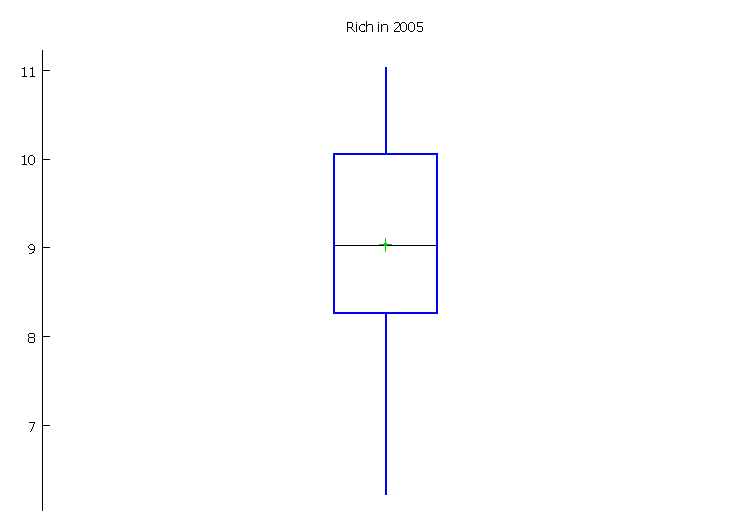
\includegraphics[scale=0.3]{parts/1a_7}
  	\label{1a:rich2005}
  }                        
  \caption{Development of income for rich countries in years 1985, 1995, 2005.}
\end{figure}

Poor countries

\begin{figure}[h!]
  \centering           
  \subfigure{                         
  	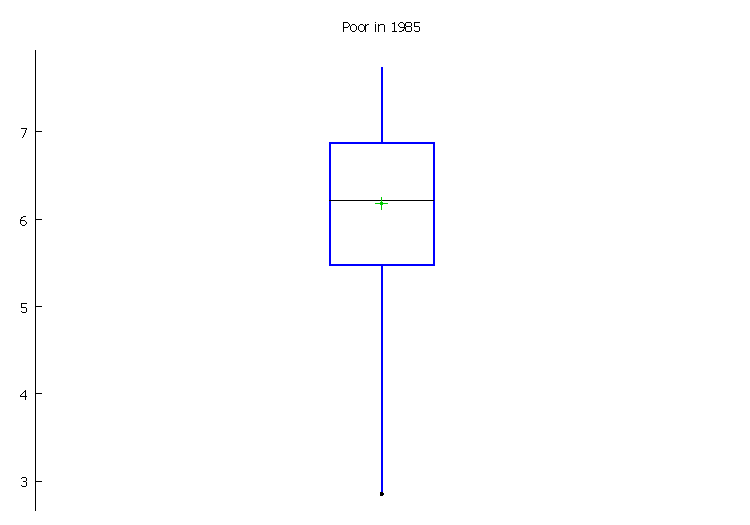
\includegraphics[scale=0.3]{parts/1a_8}
  	\label{1a:poor1985}
  }                   
  \subfigure{                         
  	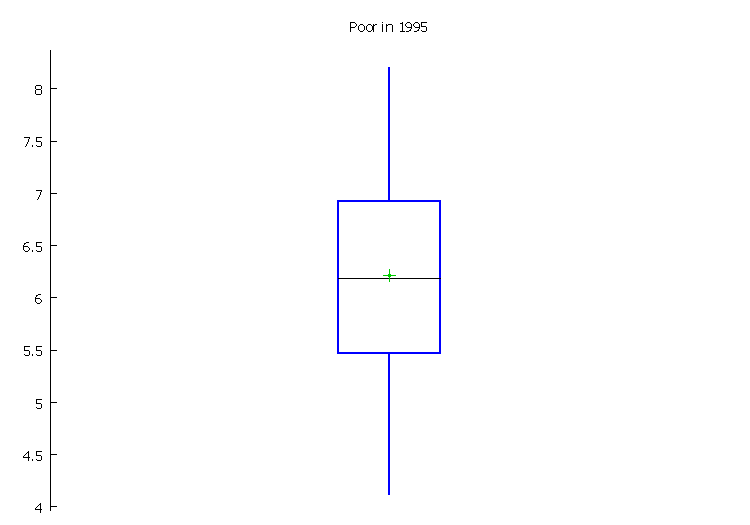
\includegraphics[scale=0.3]{parts/1a_9}
  	\label{1a:poor1995}
  }                 
  \subfigure{                         
  	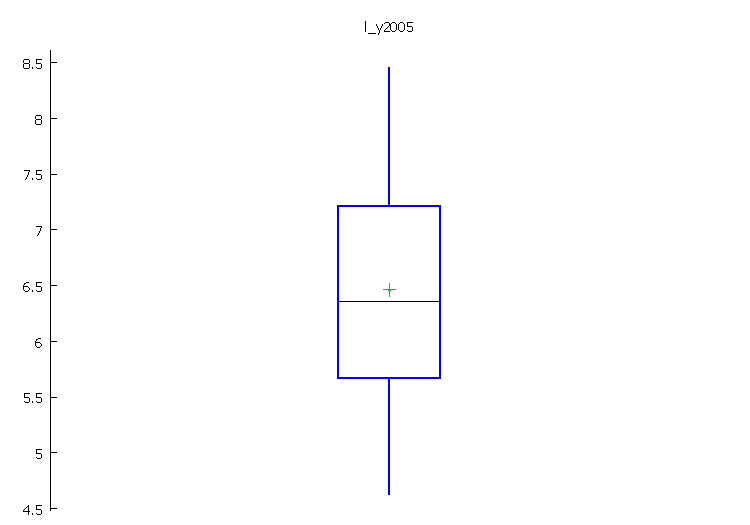
\includegraphics[scale=0.3]{parts/1a_10}
  	\label{1a:poor2005}
  }                        
  \caption{Development of income for poor countries in years 1985, 1995, 2005.}
\end{figure}

\subsection*{b) The Solow model:}



\end{document}